\documentclass[journal,12pt,twocolumn]{IEEEtran}
\usepackage{graphicx}
\graphicspath{{./figs/}}{}
\usepackage{amsmath,amssymb,amsfonts,amsthm}
\newcommand{\myvec}[1]{\ensuremath{\begin{pmatrix}#1\end{pmatrix}}}
\providecommand{\norm}[1]{\lVert#1\rVert}
\usepackage{listings}
\usepackage{watermark}
\usepackage{titlesec}
\usepackage{caption}
\let\vec\mathbf
\lstset{
frame=single, 
breaklines=true,
columns=fullflexible
}
\thiswatermark{\centering \put(0,-105.0){
\includegraphics[scale=0.15]{/sdcard/IITH/vector/vector-4/figs/logo.png}} }
\title{\mytitle}
\title{
Assignment - Vector-4
}
\author{Surajit Sarkar}
\begin{document}
\maketitle
\tableofcontents
\bigskip
\section{\textbf{Problem}}
Determine the ratio in which the line 2x+y–4=0 divides the line segment joining the points A(2,–2) and B(3,7).
\section{\textbf{Solution}}
Given $L_1$ points we get the equation
\begin{align}
    \vec{A}=\myvec{2\\-2};
\vec{B}=\myvec{3\\7} \\
-9\vec{x}+\vec{y}+20=0 ---(L_1)
\end{align}
Given $L_2$ equation
\begin{align}
    2\vec{x}+\vec{y}-4=0 ---(L_1)
\end{align}
Intersection point of $L_1$ and $L_2$
\begin{align}
    \vec{n_1}^T\vec{X}&=\vec{C}_1\\
    \vec{n_2}^T\vec{X}&=\vec{C}_2\\
    \myvec{\vec{n}_1^T\\\vec{n}_2^T}\vec{X}&=\myvec{\vec{c}_1\\ \vec{c}_2}\\
    \vec{X}&=\myvec{\vec{n}_1\\\vec{n}_2}^T\myvec{\vec{c}_1\\\vec{c}_2}\\
    &=\myvec{\frac{1}{11}&\frac{1}{11}\\ \frac{-2}{11}&\frac{9}{11}} \myvec{20\\4}\\
    &=\myvec{\frac{24}{11}\\ \frac{-4}{11}}
\end{align}
Let the ratio be k:1 and P be the point where lines intersect.\\
Using section formula
\begin{align}
\vec{P}&=\frac{k\vec{B}+\vec{A}}{k+1}\\
\frac{1}{11}\myvec{24\\-4}&=\frac{k\myvec{3\\7}+\myvec{2\\-2}}{k+1}\\
\frac{24}{11}&=\myvec{3k+2\\7k-2}\frac{1}{k+1}\\
\frac{24}{11}&=\frac{3k+2}{k+1}\\
24k+24&=33k+22\\
9k&=2\\
k&=\frac{2}{9}
\end{align}
\section{\textbf{Code Link}}
\begin{lstlisting}
https://github.com/sssurajit/fwc/blob/main/vector/vector-4/codes/vector.py
\end{lstlisting}
Execute the code by using the command\\
\textbf{python3 vector.py}
\section{\textbf{Figure}}
\begin{figure}[!h]
\centering
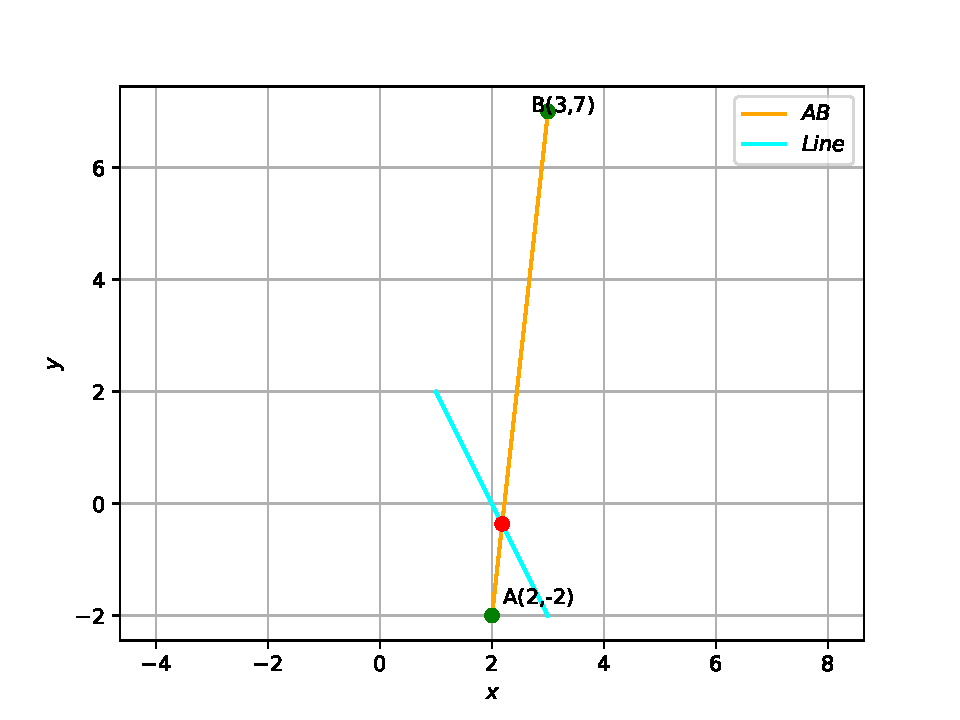
\includegraphics[width=\columnwidth]{/sdcard/IITH/vector/vector-4/figs/vec.pdf}
\caption{}
\label{fig:vec}
\end{figure}
\end{document}
